\chapter{Numerical Methods \label{cap:num}}
In this chapter, the fundamental numerical methods used to model the electromagnetic behavior in the photonic systems studied in this thesis are presented. Since most of these systems lack exact analytical solutions, especially in the absence of exploitable symmetries, numerical approaches are essential to obtain approximations with controlled precision.

The theoretical starting point is provided by the vectorial Helmholtz equations for the electric and magnetic fields, expressed in Eqs. (\ref{eqn:helmholz}) and (\ref{eqn:helmholzH}), which describe the propagation of electromagnetic waves in dielectric media. By applying the weak guidance approximation, the coupled terms on the right-hand side of both equations can be neglected. This crucial simplification eliminates cross effects between the transverse and longitudinal components of the fields, effectively decoupling the equations and reducing the complex vector problem to a set of independent scalar Helmholtz equations, which are numerically manageable. This scalar formulation is the foundation upon which the computational methods described below are implemented.
\begin{equation}
\left[\nabla^2 + k_0^2 n^2(\textbf{r})\right]\Psi(\textbf{r}) = 0 \ , \label{eqn:helmholtznum}
\end{equation}
where equation (\ref{eqn:helmholznum}) serves not only as a theoretical framework but also as the foundation for the algorithms developed in the following chapters. Its versatility allows for the adaptation of different numerical schemes according to the symmetries of the problem, as will be detailed in the subsequent sections.
\section{Eigenmode Expansion \label{cap:eme}}
This numerical method, developed and implemented during the student's Master's research, is useful when the photonic systems under study are invariantThe solutions to equation (\ref{eqn:helmholtznum}) can be expanded in plane waves with transverse profiles: $\Psi(\textbf{r}) = \Psi(x,y) \exp({i\beta z})$. With this, each transverse mode νν must satisfy the following equation to be solved numerically:
\begin{equation}
	\left[\nabla_\perp^2 + k_0^2 n^2(x,y)\right]\Psi_\nu(x,y) = \beta_\nu^2\Psi_\nu(x,y) \ , \quad\text{ con } \nabla_\perp^2 \equiv \frac{\partial^2}{\partial x^2} + \frac{\partial^2}{\partial y^2} \ .
	\label{eqn:eme}
\end{equation}
And the total propagated field is a linear combination of the modes $\Psi_\nu$: 
\begin{equation}
	\Psi(\textbf{r}) = \sum_\nu a_\nu \Psi_\nu(x,y) e^{i\beta_\nu z} \ , \quad\text{ con } a_\nu \propto \Psi_\nu(x,y) \cdot \Psi(x, y, z=0) \ . \label{eqn:emedin}
\end{equation}
Instead of directly integrating the eigenvalue equation (\ref{eqn:eme}), the strategy will be to discretize space and approximate the transverse Laplacian operator $\nabla_\perp^2$ as a matrix, since $$\frac{\partial^2 \Psi(x,y)}{\partial x^2} \sim \frac{\Psi[i+1,j]-2\Psi[i,j]+\Psi[i-1,j]}{\Delta x ^2}  \ .
$$
$\nabla^2_\perp \sim \hat{D}_{xx} \otimes I_y + I_x \otimes \hat{D}_{yy}$
The matrix is null in off-diagonal positions beyond a certain spacing (\textit{sparse-like}), so it is possible to optimize the computation process by using the Python library \href{https://docs.scipy.org/doc/scipy/reference/sparse.linalg.html}{\color{magenta}\texttt{scipy.sparse.linalg}}, specifically designed for sparse matrix linear algebra. Appendix \ref{sec:codigohelmholtz} contains an implementation of this algorithm in Python under the \href{https://www.gnu.org/licenses/gpl-3.0.html}{\color{magenta}GNU GPL v3 license}.

In Figure \ref{fig:emenumerror}, the numerical method is validated by comparison with the analytical solutions obtained in Subsection \ref{cap:solslabTETM}. The complexity of the problem is on the order of $O(N^2)$ due to the construction of the $N\times N$ matrices, which is reflected in the dependence of the execution time on the step size $\Delta x \equiv \frac{L}{N-1}$.


\begin{figure}[H]
	\centering
	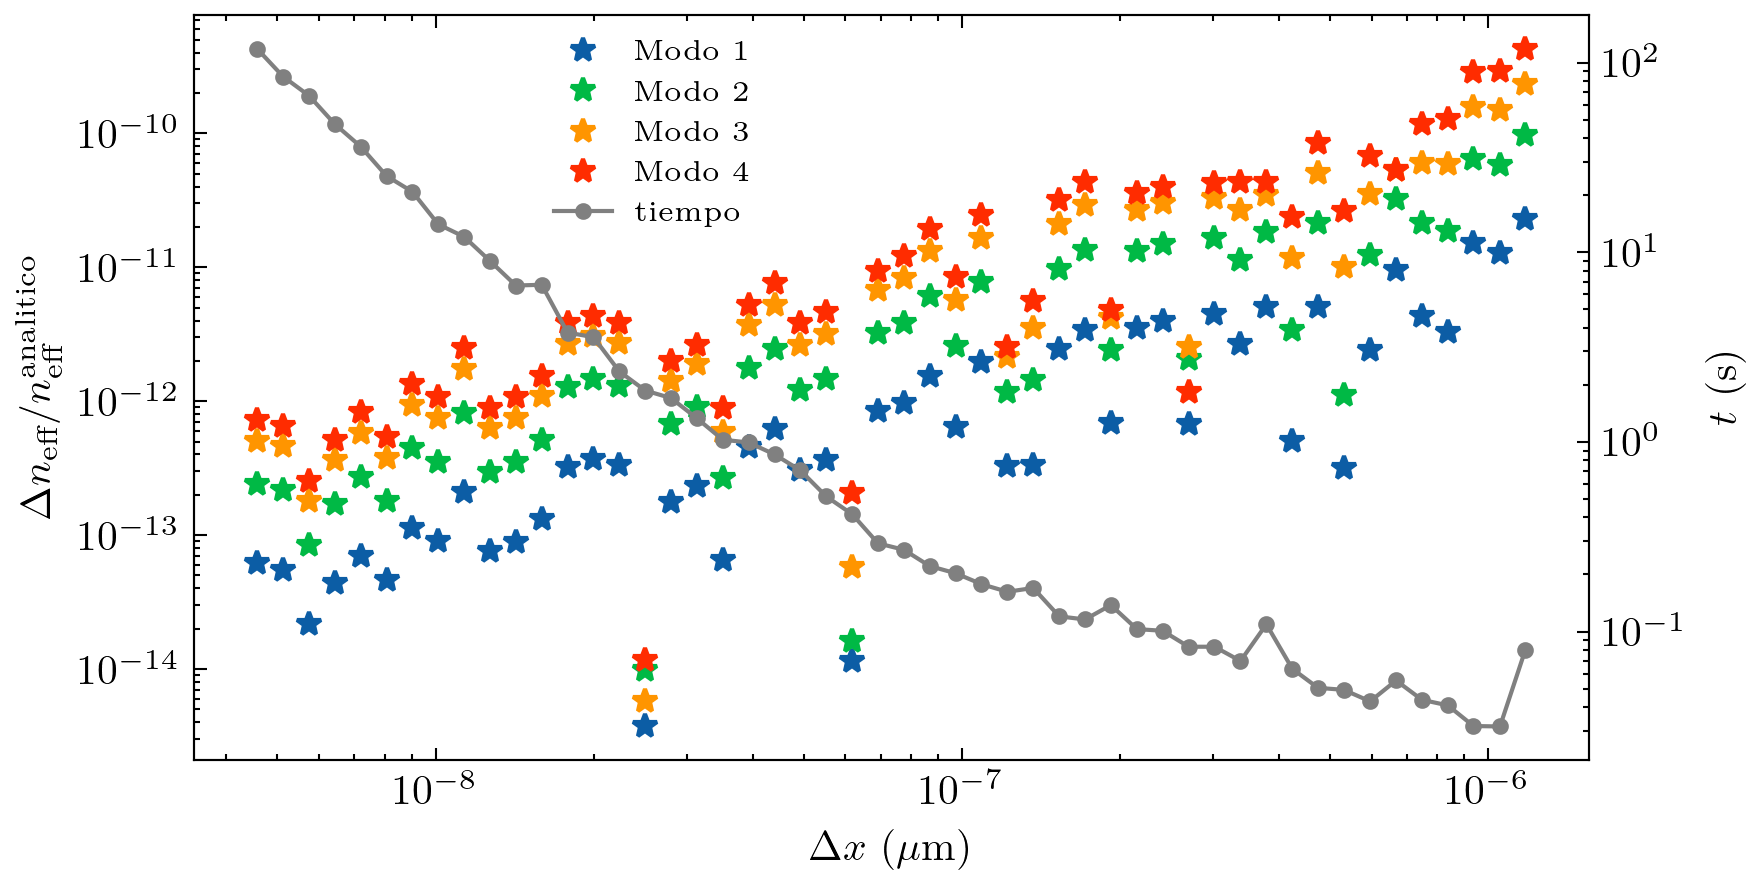
\includegraphics[width=\linewidth]{media/numerical_slab}
	\caption[Relative error and execution time.]{Relative error and execution time of the numerical solutions to equation (\ref{eqn:eme}) compared to the analytical solutions, as a function of the step size $\Delta x$. \label{fig:emenumerror}}
\end{figure}
\section{Beam Propagation Method}
Another way to approach the numerical integration of equation (\ref{eqn:helmholtznum}) involves separating the field into its slow envelope and a rapidly oscillating phase, considering that in the visible range the order of magnitude is $k_0 \sim 10 ^{5} \text{ cm}^{-1}$: $\Psi(\textbf{r}) = \phi(x,y,z)\exp(ik_0 n_0 z)$. After substituting into equation (\ref{eqn:helmholtznum}), the optical Schrödinger equation is obtained \citep{paraxialschrodinger}:
\begin{equation}
	-2ik_0 n_0\frac{\partial }{\partial z}\phi(x,y, z) =  \left[\nabla_\perp^2 + k_0^2 (n^2(\textbf{r})-n_0^2)\right]\phi(x,y, z) \ , \label{eqn:bpmescalar}
\end{equation} 
where the paraxial approximation $\left| \frac{\partial^2 \phi}{\partial z^2} \right| \ll 2 k_0 n_0\left| \frac{\partial \phi}{\partial z} \right|$has been used. Algorithms that solve equation (\ref{eqn:bpmescalar}) are known as scalar Beam Propagation Methods (BPM), widely used in this research area \cite{bics, interorbital, OAMCaging, vortex, bpm}. Outside the weak guidance approximation, cross-polarization effects become more relevant, and a vectorial description of the problem is necessary.
\subsection{Implementation via Fourier Transform (FFTBPM)}
Equation (\ref{eqn:bpmescalar}) can be written in terms of linear differential operators as \citep{bpm}:
\begin{equation}
	\frac{\partial \phi}{\partial z}  = \left(\hat{A} + \hat{B}\right)\phi, \text{ con } \hat{A} \equiv i\frac{\nabla^2_\perp}{2k_0n_0}\text{ y } \hat{B} \equiv i\frac{k_0}{2n_0}\left[n^2(\textbf{r})-n_0^2\right] \ . \label{eqn:bpmop}
\end{equation}
The formal solution to equation (\ref{eqn:bpmop}) is $\phi(\textbf{r}) = \exp\left[\left(\hat{A} + \hat{B}\right)(z-z_0)\right]\phi(x, y, z_0)$. It is convenient to work with the operator \( \hat{A} \) in Fourier space and the operator \( \hat{B} \) in real space. This is because \( \hat{A} \) contains spatial derivatives—in particular, the transverse Laplacian operator \( \nabla^2_\perp \)— which become simple multiplications upon applying the Fourier transform. Thus, the operation \( \hat{A} \phi \) becomes computationally efficient when transformed into the wavevector domain \( \textbf{k}_\perp \), where it acts as a diagonal operator. On the other hand, \( \hat{B} \) depends on the spatial profile of the refractive index \( n(\textbf{r}) \), which is defined locally in real space. Evaluating this term in Fourier space would involve a convolution, which is unnecessarily costly and less intuitive. For this reason, it is kept in real space.

Since $\hat{A}$ and $\hat{B}$ do not commute in general, the exponential operator can be expanded to order $O(\Delta z ^3)$ as $\exp\left[\left(\hat{A} + \hat{B}\right)\Delta z \right] \approx \exp\left(\frac{\hat{A}\Delta z}{2} \right)\exp\left(\hat{B}\Delta z \right)\exp\left(\frac{\hat{A}\Delta z}{2} \right) + O(\Delta z ^3)$.

The algorithm implemented in Appendix \ref{sec:codeBPM} is as follows: \begin{enumerate}
	\item Start with a profile $\phi(x, y, z_0)$
\item Act in Fourier space by transforming the profile and multiplying by the phase associated with $\hat{A}$: $\exp\left(\frac{ik^2\Delta z}{4k_0 n_0}\right)\mathcal{F}(\phi(z_0))$, where $k=\sqrt{k_x^2 + k_y^2}$ are the Fourier frequencies.
\item Apply the inverse Fourier transform and multiply by the phase associated with $\hat{B}$: 

$\exp\left[\frac{i\Delta z k_0^2(n^2-n_0^2)}{2 k_0n_0}\right]\mathcal{F}^{-1}\left(\exp\left(\frac{ik^2 \Delta z}{4k_0 n_0}\right)\mathcal{F}(\phi(z_0))\right)$
\item Return to Fourier space and multiply by the phase associated with $\hat{A}$:
 
$\exp\left(\frac{ik^2\Delta z}{4k_0 n_0}\right)\mathcal{F}\left\{\exp\left[\frac{ik_0^2(n^2-n_0^2)}{2 k_0n_0}\Delta z \right]\mathcal{F}^{-1}\left[\exp\left(\frac{ik^2\Delta z}{4k_0 n_0}\right)\mathcal{F}(\phi(z_0))\right]\right\}$
\item Return to real space, having advanced one step $\Delta z$:

$\phi(z_0+\Delta z)=\mathcal{F}^{-1}\left\{\exp\left(\frac{ik^2\Delta z}{4k_0 n_0}\right)\mathcal{F}\left\{\exp\left[\frac{i k_0^2(n^2-n_0^2)}{2 k_0n_0}\Delta z\right]\mathcal{F}^{-1}\left[\exp\left(\frac{ik^2\Delta z}{4k_0 n_0}\right)\mathcal{F}(\phi(z_0))\right]\right\} \right\}$

\item Iterate until the desired propagation distance zz is reached.
\end{enumerate} Figure \ref{fig:num-exp-comp} compares experimental results with numerical simulations obtained via BPM. The normalized intensity profiles show remarkable qualitative agreement, particularly in the spatial distribution of the main lobes.

\begin{figure}[H]
	\centering
	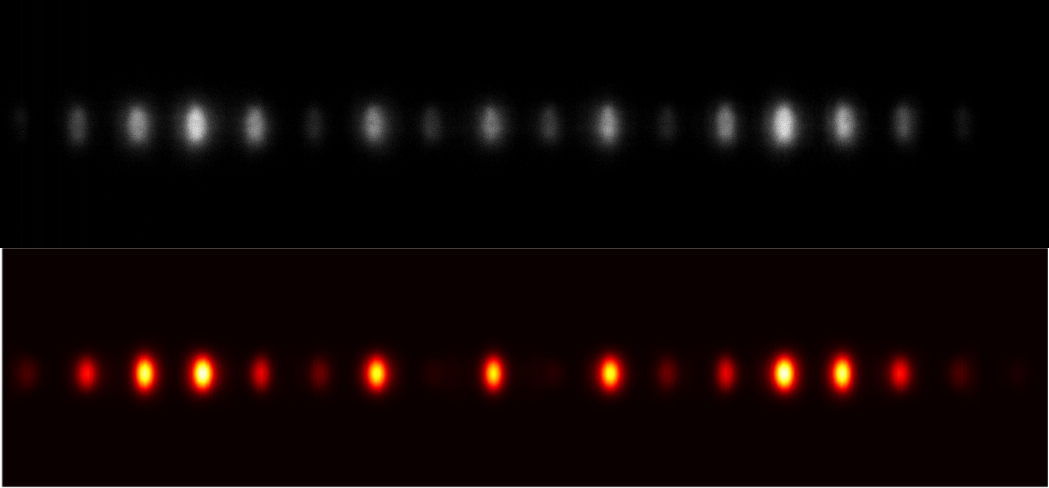
\includegraphics[width=\linewidth]{media/num_exp_comparison.png}
	\caption[Excitation of the central site of a one-dimensional lattice.]{Excitation of the central site of a one-dimensional lattice.
		\textbf{Top:} Experimental measurement at $\lambda$ = 730 nm.
textbf{Bottom:} Numerical simulation performed with BPM.
\label{fig:num-exp-comp}} \end{figure} This level of qualitative agreement validates the weak guidance approximation used in equation (\ref{eqn:helmholtznum}), as well as the paraxial approximation, and reinforces the reliability of the numerical method for designing photonic devices with analogous geometries.

\section{Comments on Coupled-Mode Theory \label{cap:CMT}}
The numerical simulation of equations (\ref{eqn:non-ortho-CMT-eqs}) represents the most compact formulation possible, since the coupling matrix $\hat{C} \equiv \hat{P}^{-1}\hat{H}$ encodes all the properties of the network to be studied in a semi-empirical manner. In this sense, the diagonalization of $\hat{C}$ constitutes a valuable numerical tool for analyzing the behavior of photonic networks under variations of parameters such as dimerization (defined as the ratio between two coupling constants) or detuning (the difference between the propagation constants of distinct modes).

Furthermore, this approach allows for the exploration of even "non-physical" systems, thanks to the degrees of freedom available in the elements of $\hat{C}$: for example, cases where second-neighbor coupling is greater than first-neighbor coupling, or systems with complex couplings.

In the weak guidance approximation, the longitudinal components of the electric field can be neglected:
\[ \nabla \cdot (n^2 \textbf{E}) \overset{\nabla n^2 \sim 0}{\sim} n^2 \nabla \cdot \textbf{E} = 0 \ ,\]
where the order of magnitude of the longitudinal field component is $|E_z| \sim |\nabla_\perp \cdot \textbf{E}_\perp|/\beta$. Thus, the studied modes are quasi-transverse, and the matrix $\hat{P}$ reduces to:
\begin{equation}
    P_{ij} \sim \frac{k_z^i + k_z^j}{4\omega\mu_0} \iint \left(\textbf{e}_i^\perp\right)^* \cdot \textbf{e}_j^\perp dxdy \ .
    \label{eqn:CMTnum}
\end{equation}
Equation (\ref{eqn:CMTnum}), which quantifies the overlap between modes, along with equation (\ref{eqn:hij}) describing the matrix elements of the Hamiltonian operator, constitute fundamental tools for the comparative analysis between the Eigenmode Expansion (EME) method and Coupled-Mode Theory (CMT). This comparison is performed through a systematic study of the eigenvalue spectrum of the coupling matrix $\hat{C}$, which contains essential information about the effective propagation constants of the system.

Figure \ref{fig:EMECMT} presents a quantitative analysis of this comparison, showing the evolution of the eigenvalues for a dielectric photonic coupler as a function of the separation distance between waveguides. It is observed that both methods converge asymptotically for distances greater than $d > 20\,\mu$m, where the weak field approximation of CMT holds. However, in the strong coupling regime ($d < 13\,\mu$m), discrepancies begin to become noticeable.

Beyond the spectral analysis, the validity of the computed eigenstates can be indirectly verified through equation (\ref{eqn:emedin}), which relates the field evolution to the projection onto the system's eigenmodes, and by qualitatively comparing the dynamic profiles obtained with the experimental and numerical results shown in Figure \ref{fig:num-exp-comp}. This analysis (see Figure \ref{fig:1darraycmt}) allows establishing the applicability limits of each numerical method: while EME provides accurate results across the entire parameter range at the cost of higher computational complexity, CMT offers an efficient alternative for weakly coupled systems where the approximation of localized modes remains valid: separation distances $d \gtrapprox$ 15 $\mu$m.
\begin{figure}[h]
    \centering
    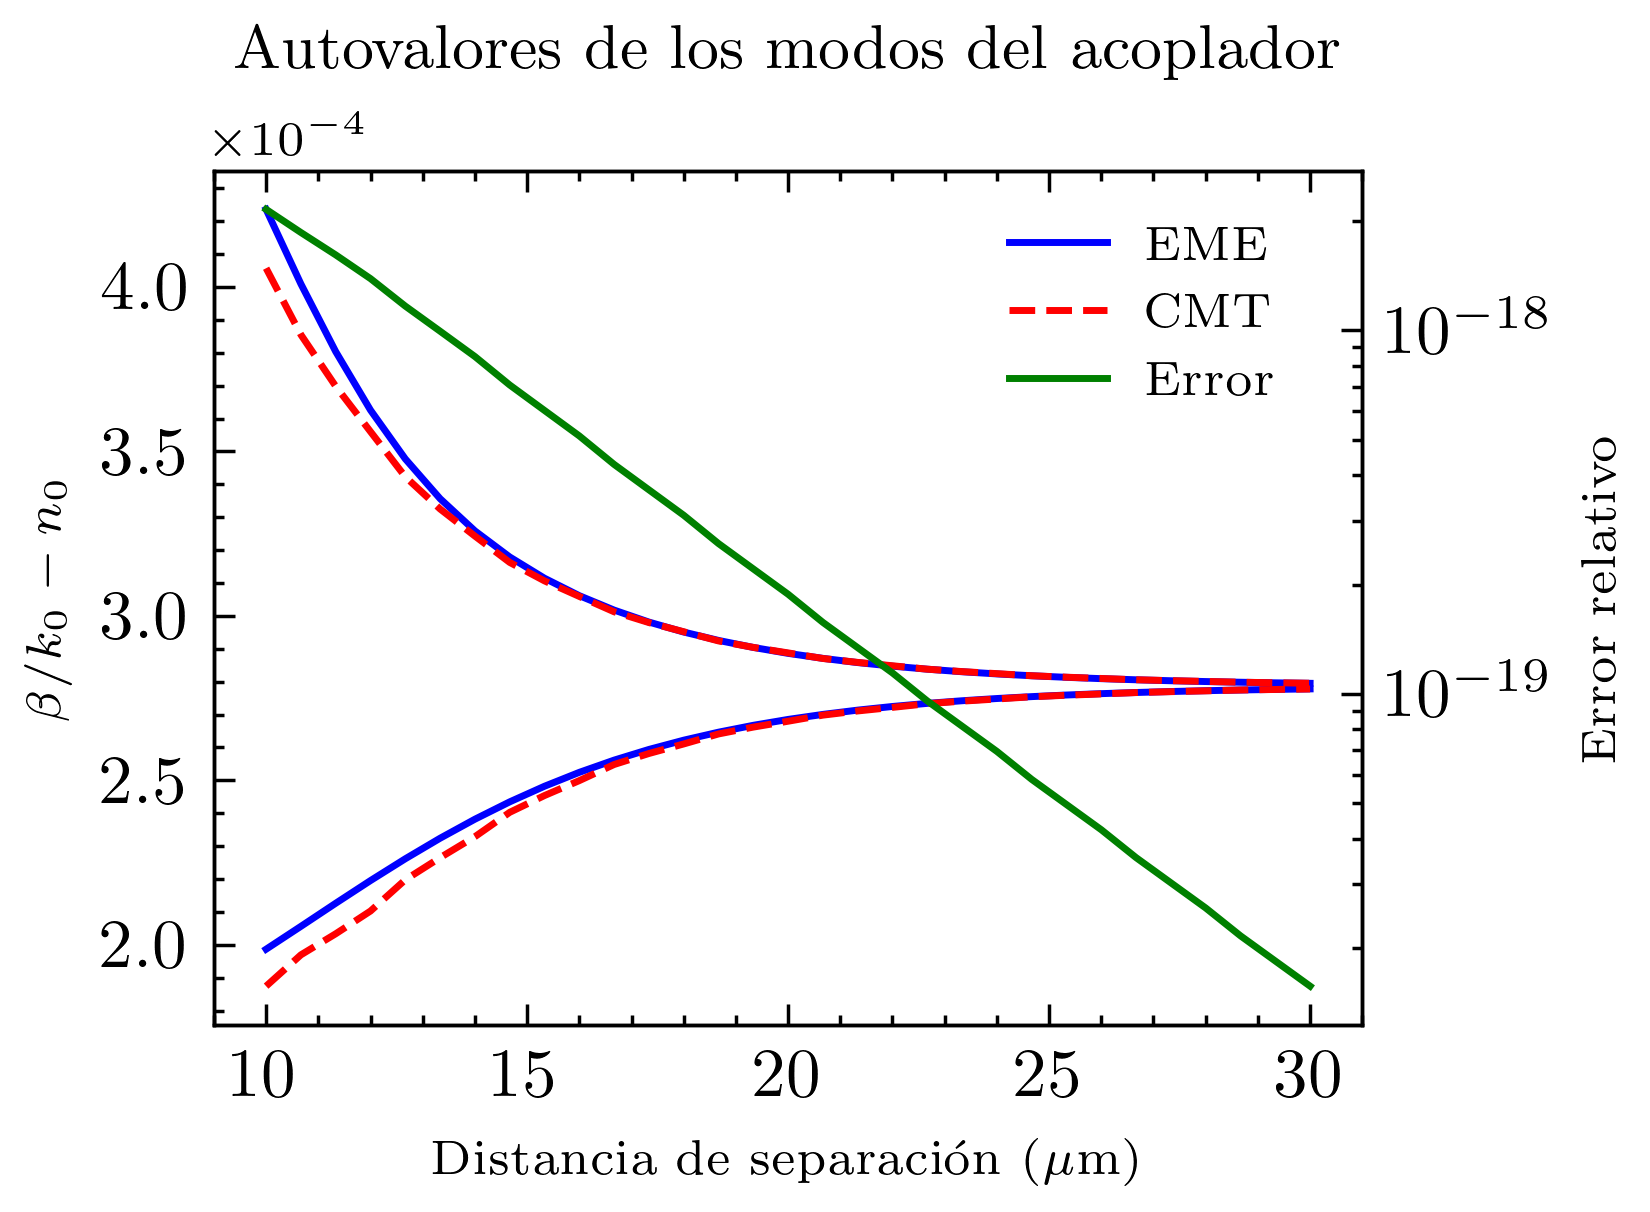
\includegraphics[width=0.8\linewidth]{codigo/dimol/coupler.png}
    \caption[Comparison between EME and CMT.]{Comparison of the eigenvalues obtained with the Eigenmode Expansion (EME) method and with Coupled-Mode Theory (CMT). Greater divergence is observed when the distance between waveguides is small. Parameters used: $n_0=1.48$, $\Delta n = 4\times10^{-4}$, $\lambda = 730$ nm y $a = 3\,\mu$m.}
    \label{fig:EMECMT}
\end{figure}
\begin{figure}[h]
	\centering
	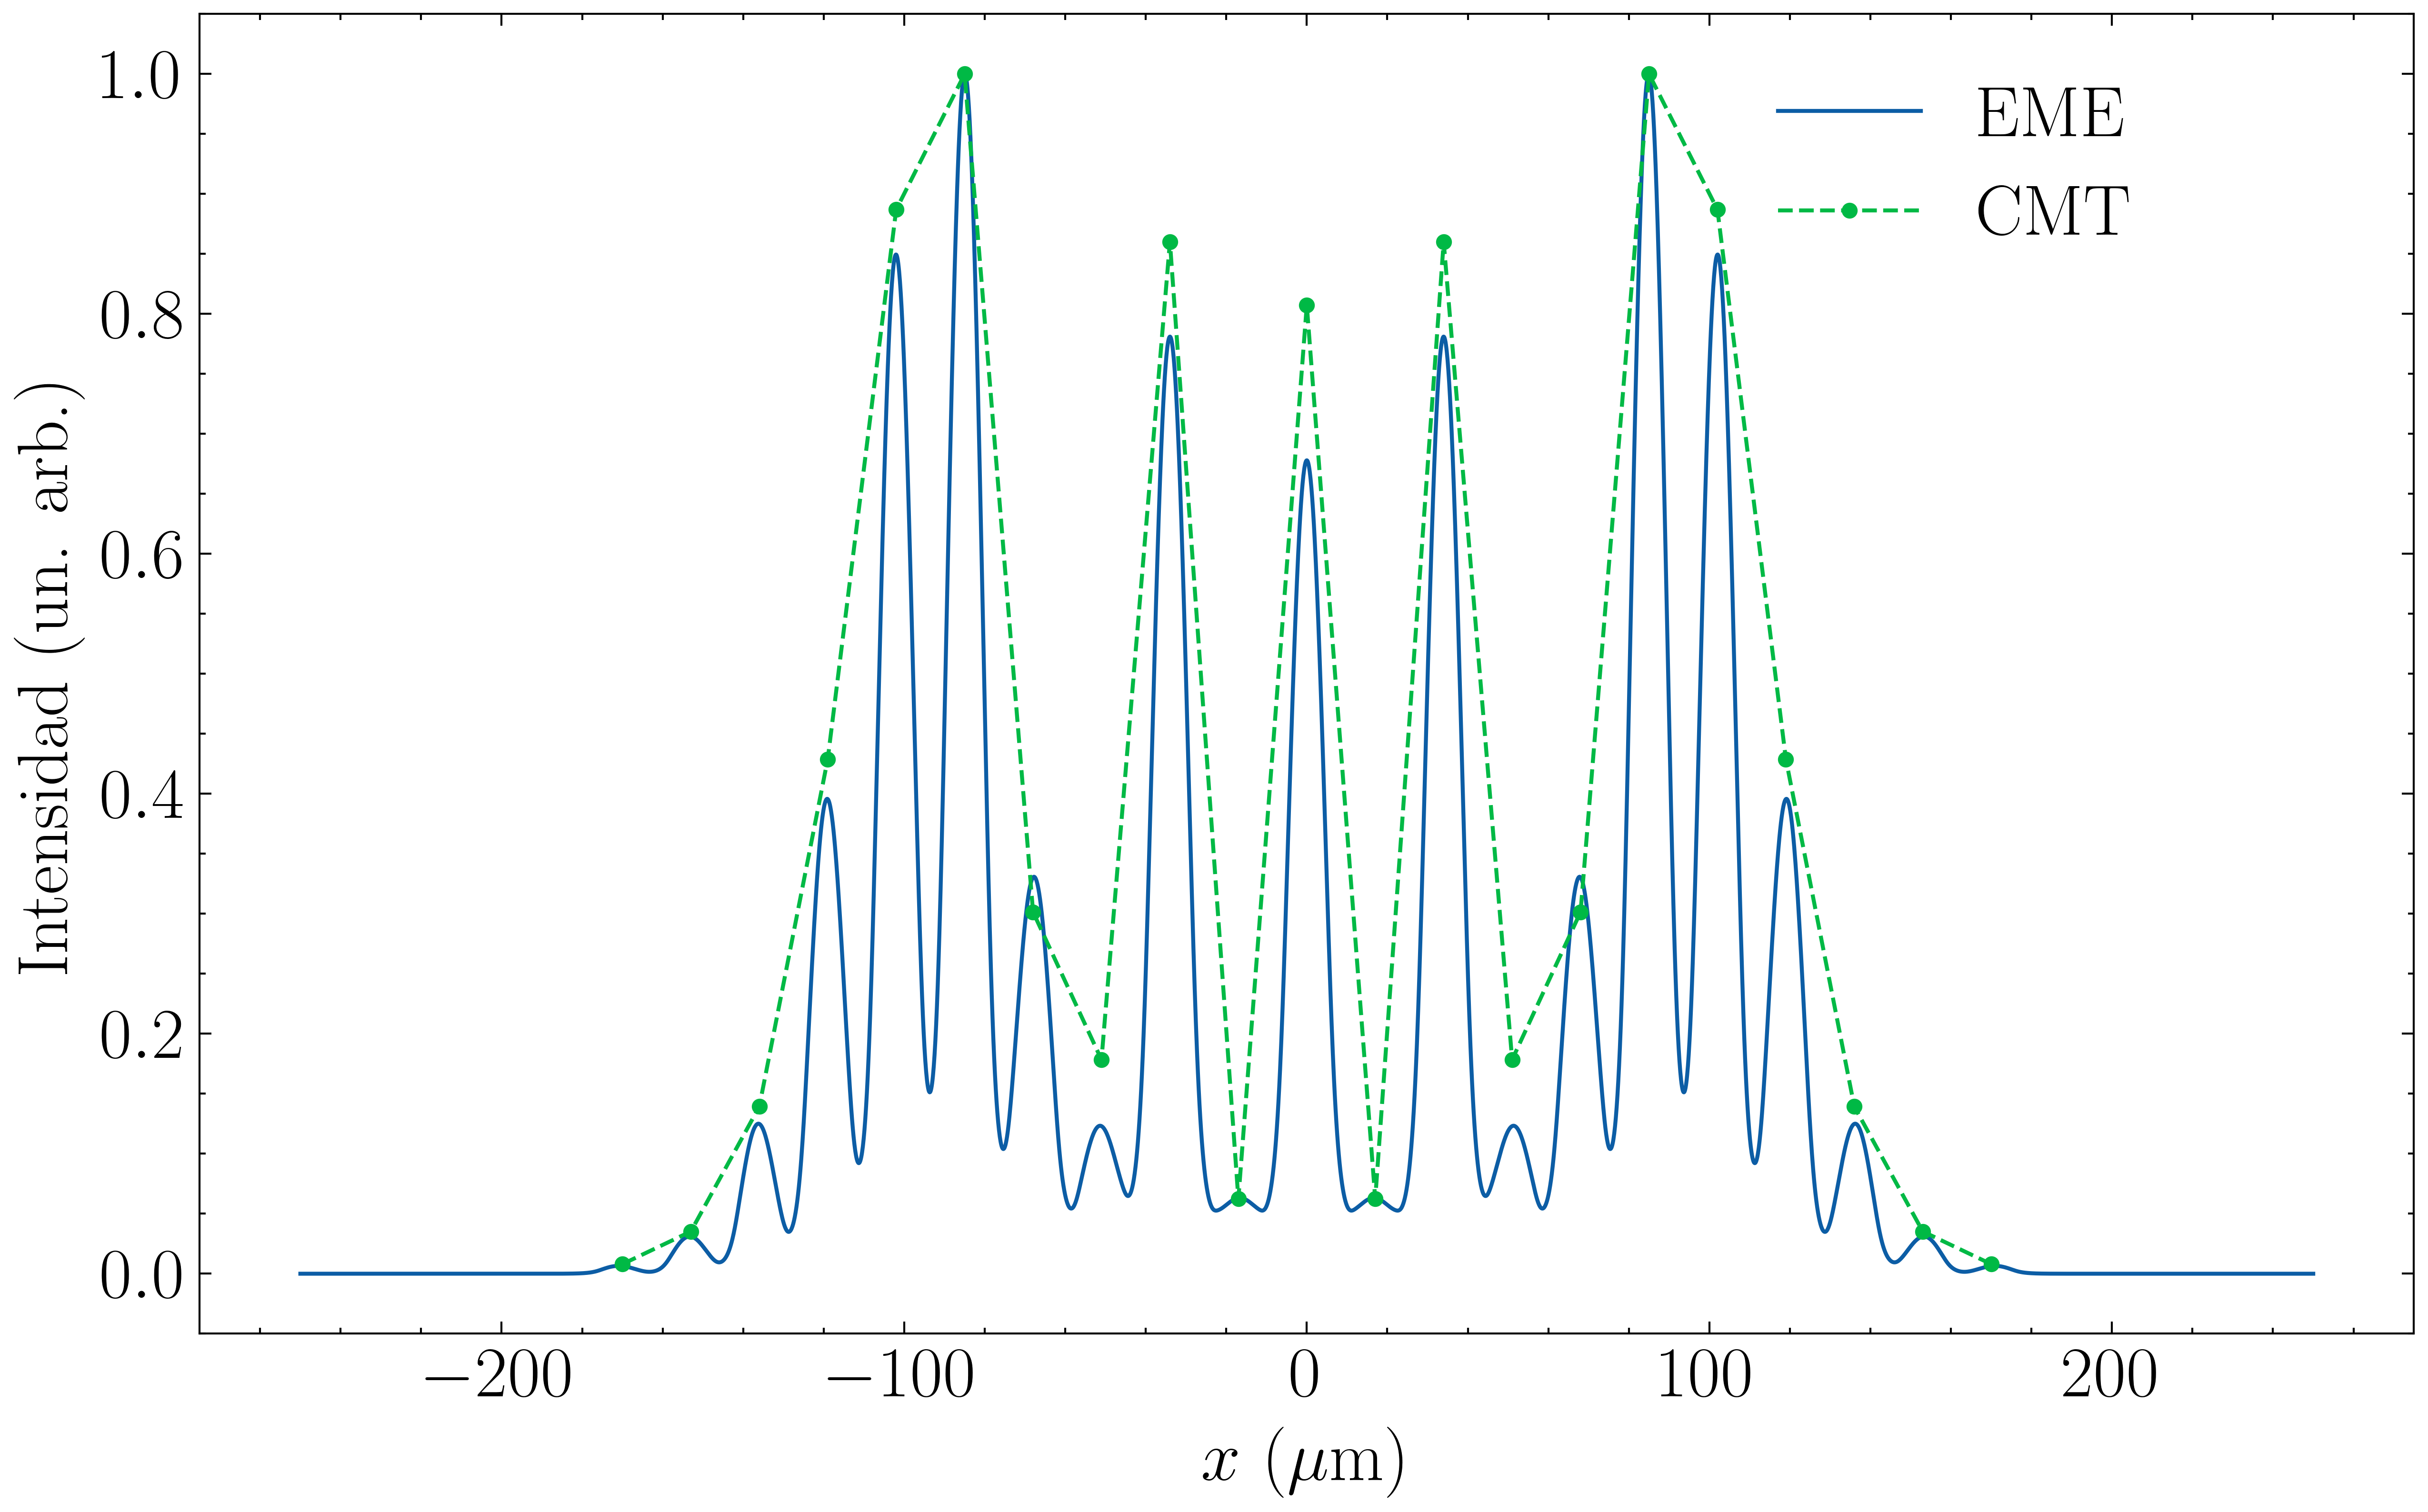
\includegraphics[width=0.8\linewidth]{codigo/1darraycmt/1darraycmt.png}
	\caption[Dynamics with EME and CMT.]{Dynamic profile of a one-dimensional array of 21 waveguides at a distance $d=17$ $\mu$m simulated with CMT and with EME. The results are similar to those in Figure \ref{fig:num-exp-comp}.}
	\label{fig:1darraycmt}
\end{figure}
